\subsection{Semantic Multi-Modal Frame Representation}
We represent the each frame of input videos as in terms of set of language and visual atoms. Language atoms are the salient words detected via ranking tf-idf like measure, and the visual atoms are found via clustering over object proposals which we extract from frames. We explain the details of finding the atoms and representing the frames in the subsequent sections.
\subsubsection{Learning Language Atoms}
In order to detect the salient words, we use tf-idf like measure. For each recipe, we concatanate all subtitles into a single term corpus. As a document corpus, we use all the words extracted from all recipes. Moreover, we compute the tf-idf as $tfidf(w,d,D)=f_{w,d} \times \log \frac{N}{n_{w}}$ where $w$ is the word, $d$ is the corpus of the recipe, $f_{w,d}$ is the frequency of the word in the recipe, $N$ is the total number of videos in all recipes and $n_{w}$ is the number of videos whose subtitle include the word $w$. After computing the tf-idf, we sort all words with their tf-idf values and choose top $K$ words as set of salient words (\emph{We set $K=100$ in our experiments}).
\subsubsection{Learning Visual Atoms}
In order to learn visual atoms, we initially generate object proposals from each frame of each videos. This proposals are generated by using apperance and motion cues via the Constrained Parametric Min-Cut (CPMC) \cite{cpmc} algorithm. We apply CPMC algorithm to each frame of the each video returned by the query independently and create a collection of region proposals. We note the $k^{th}$ region of $t^{th}$ frame of $i^{th}$ video as $r^{(i),k}_t$. Moreover, we drop the video index $(i)$ if it is clear from the context.

We follow the spectral graph clustering approach in order to group these regions into semantically meaningful objects similar to the KeySegments by Lee et al.\cite{keysegments}. Moreover, idea of clustering region proposals into semantic objects have been mostly utilizied for clusters generated by a single video and they fail to cluster objects having a large visual difference. Hence, we extend this work to spectral joint clustering of region proposals.

\paragraph{Joint Proposal Clustering to Detect Visual Objects}
Since our proposals are generated from multiple videos, combining them into a single region collection and clustering it is not desired for two reaons; (1) the objects have large visual differences among different videos and accurately clustering them into a single object is hard, (2) objects clusters are desired to have region proposals from multiple videos in order to relate videos easily. Hence, we propose a joint version of the spectral region clustering algorithm.

\begin{figure}[ht]
  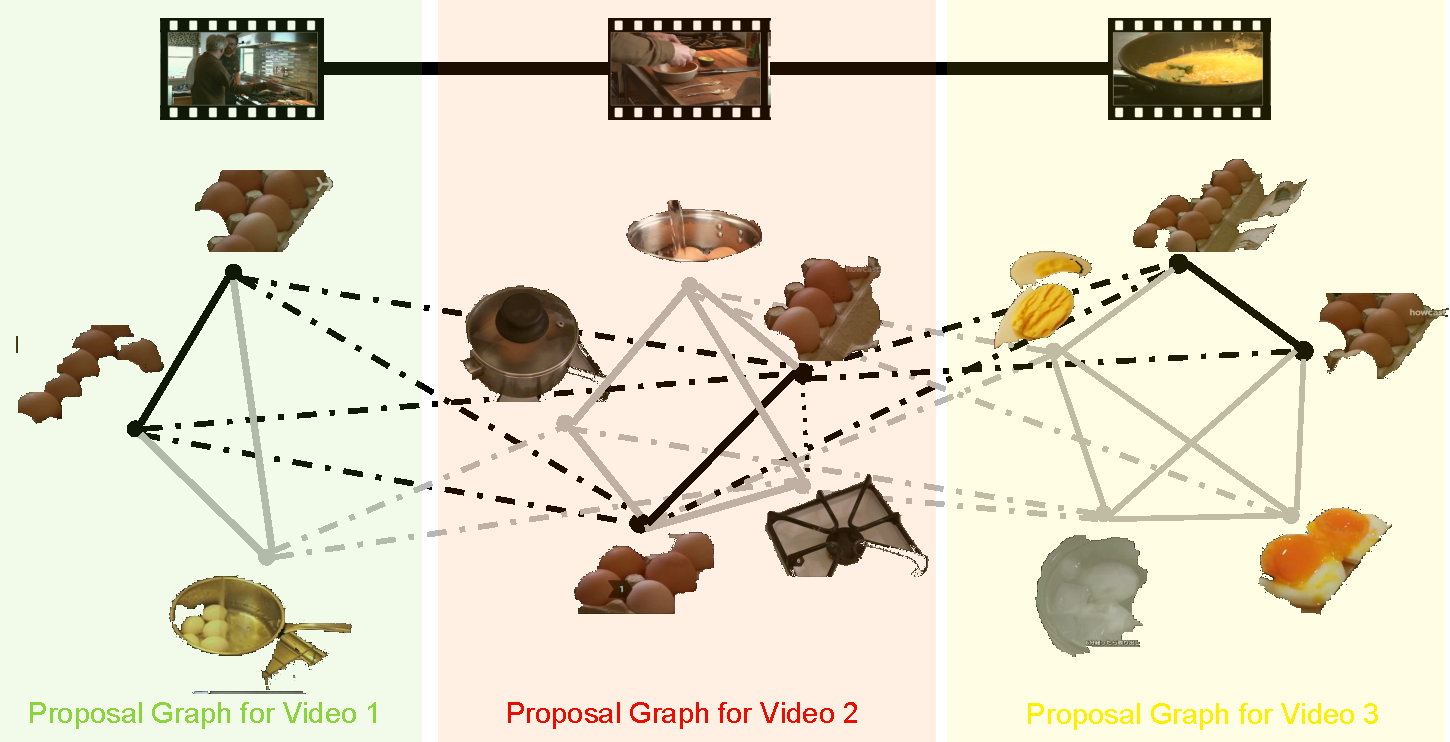
\includegraphics[width=0.48\textwidth]{joint_clustering}
  \scalebox{0.85}{$\arg\max  \color[HTML]{BF9000}{\frac{x_1^TA^{(1)}x^1}{x_1^Tx^1}}+\color[HTML]{990000}{\frac{x_2^TA^{(2)}x^2}{x_2^Tx^2}}+\color[HTML]{38761d}{\frac{x_3^TA^{(3)}x^3}{x_3^Tx^3}}+\color[HTML]{a64d79}{\frac{x_1^TA^{(1,2)}x^2}{x_1^T\mathds{1}\mathds{1}^Tx^2}}+\color[HTML]{F1C232}{\frac{x_2^TA^{(2,3)}x^3}{x_2^T\mathds{1}\mathds{1}^Tx^3}}$}
  \caption{Visualization of the joint proposal clustering.}
  \label{hierProposal}
\end{figure}

Here, we first explain the original spectral graph clustering algorithm and then extend it to our joint version. Consider set of region proposals extracted from a single video $r^k_t$, and a similarity metric $d(\cdot,\cdot)$ which assigns similarity between each region pair. We follow the Single Cluster Graph Partitioning (SCGP)\cite{scgp} to find the dominant cluster which maximizes the inter-cluster similarity. In other words, we solve
\begin{equation}
  \argmax \frac{\sum_{(k_1,t_1),(k_2,t_2) \in K \times T} x^{k_1}_{t_1} x^{k_2}_{t_2} d(r^{k_1}_{t_1},r^{k_2}_{t_2})}{\sum_{(k,t) \in K \times T} x^{k}_t}
\end{equation}
Where, $x^{i,k}_t$ is a binary variable which is $1$ if $r^{(i),k}_t$ is included in the cluster. Moreover, we drop the video index for clarity. When we use the vector form of the indicator variables as $\mathbf{x_{tK+k}}=x^{k}_{t}$ and the pairwise distance matrix as $\mathbf{A}_{t_1K+k_1,t_2K+k_2}=d(r^{k_1}_{t_1},r^{k_2}_{t_2})$, this equation can be compactly written as
$\argmax_{\mathbf{x}} \frac{\mathbf{x^T}A\mathbf{x}}{\mathbf{x^T}\mathbf{x}}$
Moreover, it can be solved by computing the dominant eigenvector of $\mathbf{x}$ after relaxing it to $[0,1]$ from binary \cite{scgp,scgp_eigen}. After finding the maximum, the remaining clusters can be found by removing the selected region proposals from the collection, and re-aplying the same algorithm for the second dominant cluster.

Our extension of the SCGP into multiple videos is based on the assumption that the dominant objects occur in most of the videos. Hence, we re-formulate the problem by relating videos to each other. We start with creating the kNN graph of videos based on their language description similarities. Moreover, we also create the kNN graph of region proposals in each video. This hierarchical graph structure is visualized in Figure~\ref{hierProposal}. After creating this graph, we impose the similarity of regions coming from each video as well as the similarity of regions coming from neighbour videos. Hence, given the pairwise distance matrix $\mathbf{A^(i)}$, binary indicator vectors $\mathbf{x^(i)}$ for each video and pairwise distance matrices for video pairs as $\mathbf{A^{(i,j)}}$, we define our optimization problem as;
\begin{equation}
\argmax \sum_{i \in N} \frac{\mathbf{x^{(i)^T}}\mathbf{A^{(i)}}\mathbf{x^{(i)}}}{\mathbf{x^{(i)^T}}\mathbf{x^{(i)}}} +
\sum_{i \in N} \sum_{j \in \mathcal{N}(i)} \frac{\mathbf{x^{(i)^T}}\mathbf{A^{(i,j)}}\mathbf{x^{(j)}}} {\mathbf{x^{(i)^T}}\mathds{1}\mathds{1}^T\mathbf{x^{(j)}}}
\end{equation}
where $\mathcal{N}(i)$ is the neighbours of the video $i$ in the kNN graph and $\mathds{1}$ is vector of ones. We visualize this optimization objective in Figure~\ref{hierProposal} for the case of 3 videos and 1-NN video graph, 2-NN region proposal graph.

After changing the optimization function, we can not use the efficient eigen-decomposition based approach from \cite{scgp,scgp_eigen}; however, we can use stochastic gradient descent (SGD) since the cost function is quasi-convex when it is relaxed. Hence, we use SGD with the following gradient function;
\begin{equation}
  \text{Some vector matrix multiplication}
\end{equation}

In Figure~\ref{cvis}, we visualize some of the clusters which our algorithm generated after applied on the videos returned by the query \emph{How to Hard Boil an Egg}. As shown the figure, the resulting clusters are highly correlated and correspond to semantic objects\&concepts.
\begin{figure}[ht]
  \begin{subfigure}[b]{0.23\textwidth}
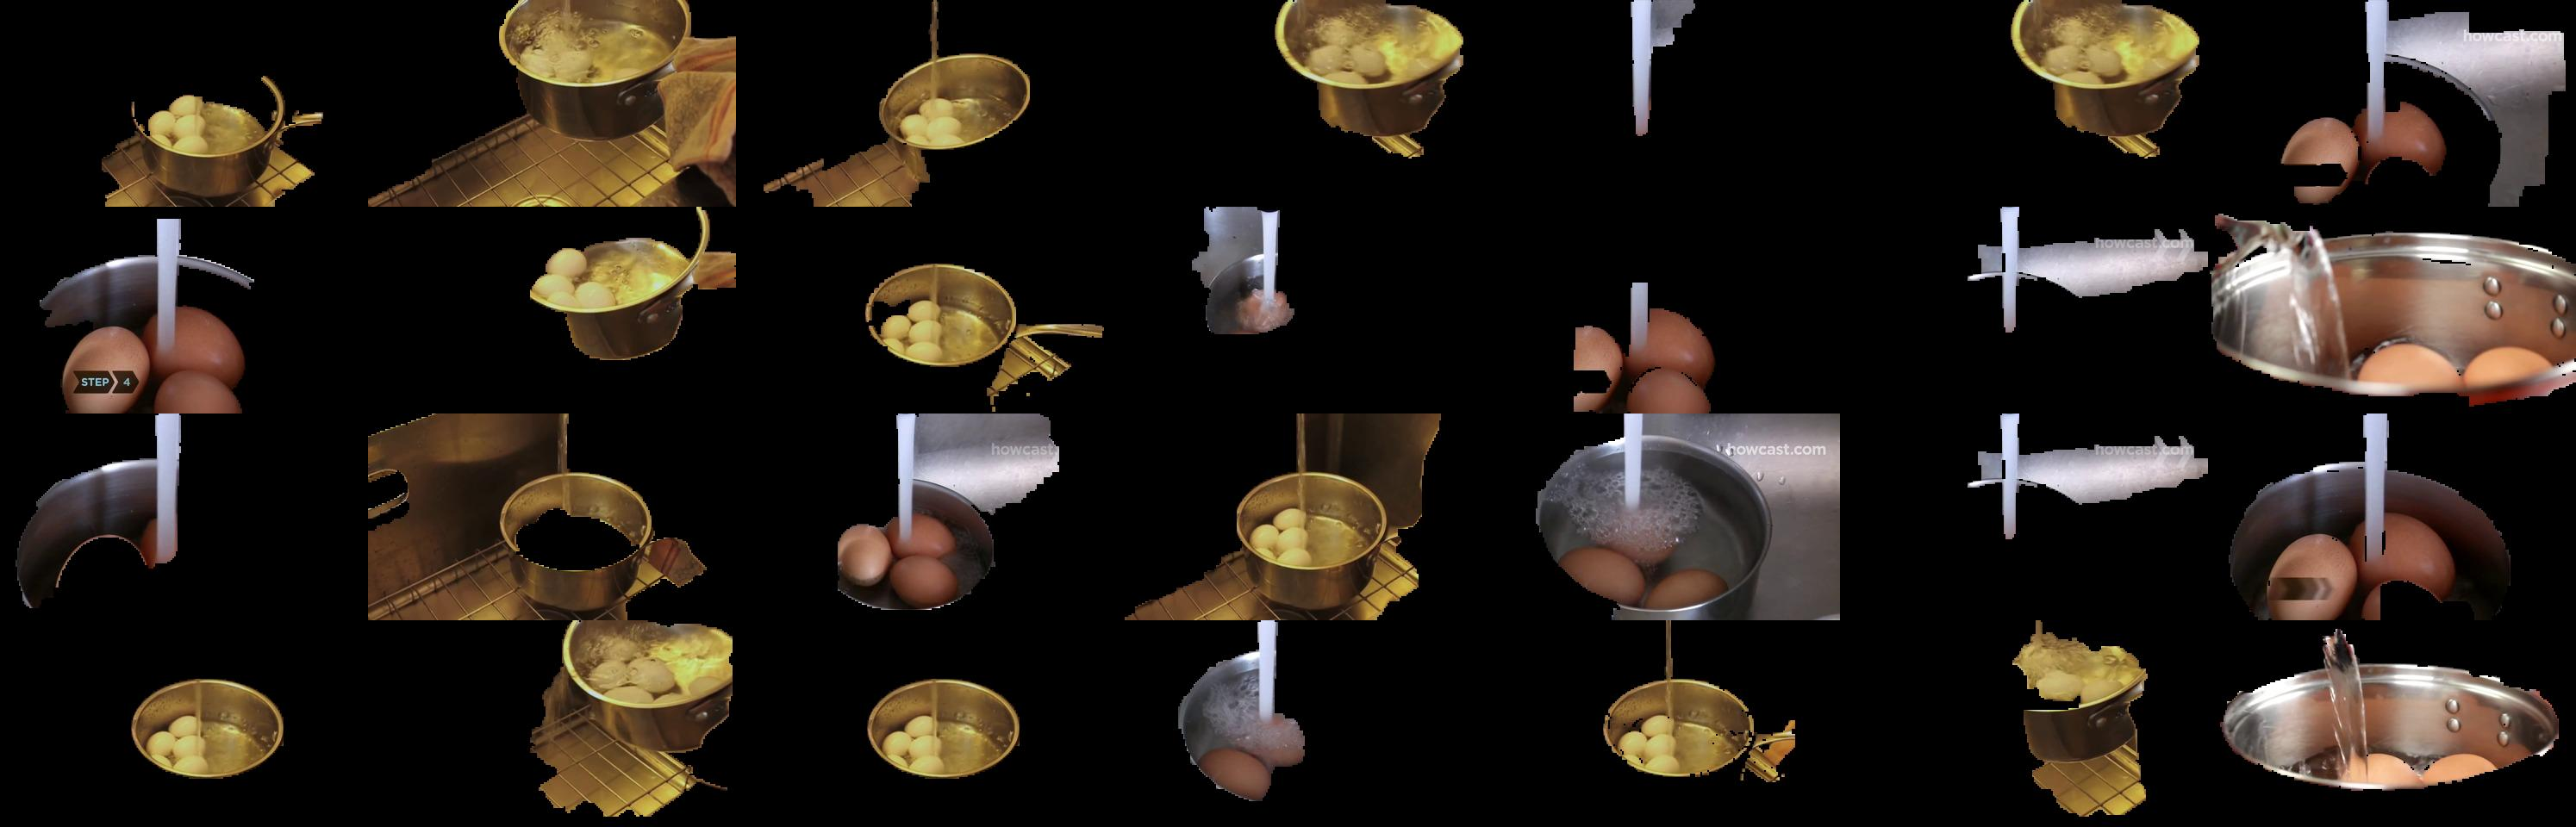
\includegraphics[width=\textwidth]{im0.png}
%\caption{Cluster 1}
\end{subfigure}
~
\begin{subfigure}[b]{0.23\textwidth}
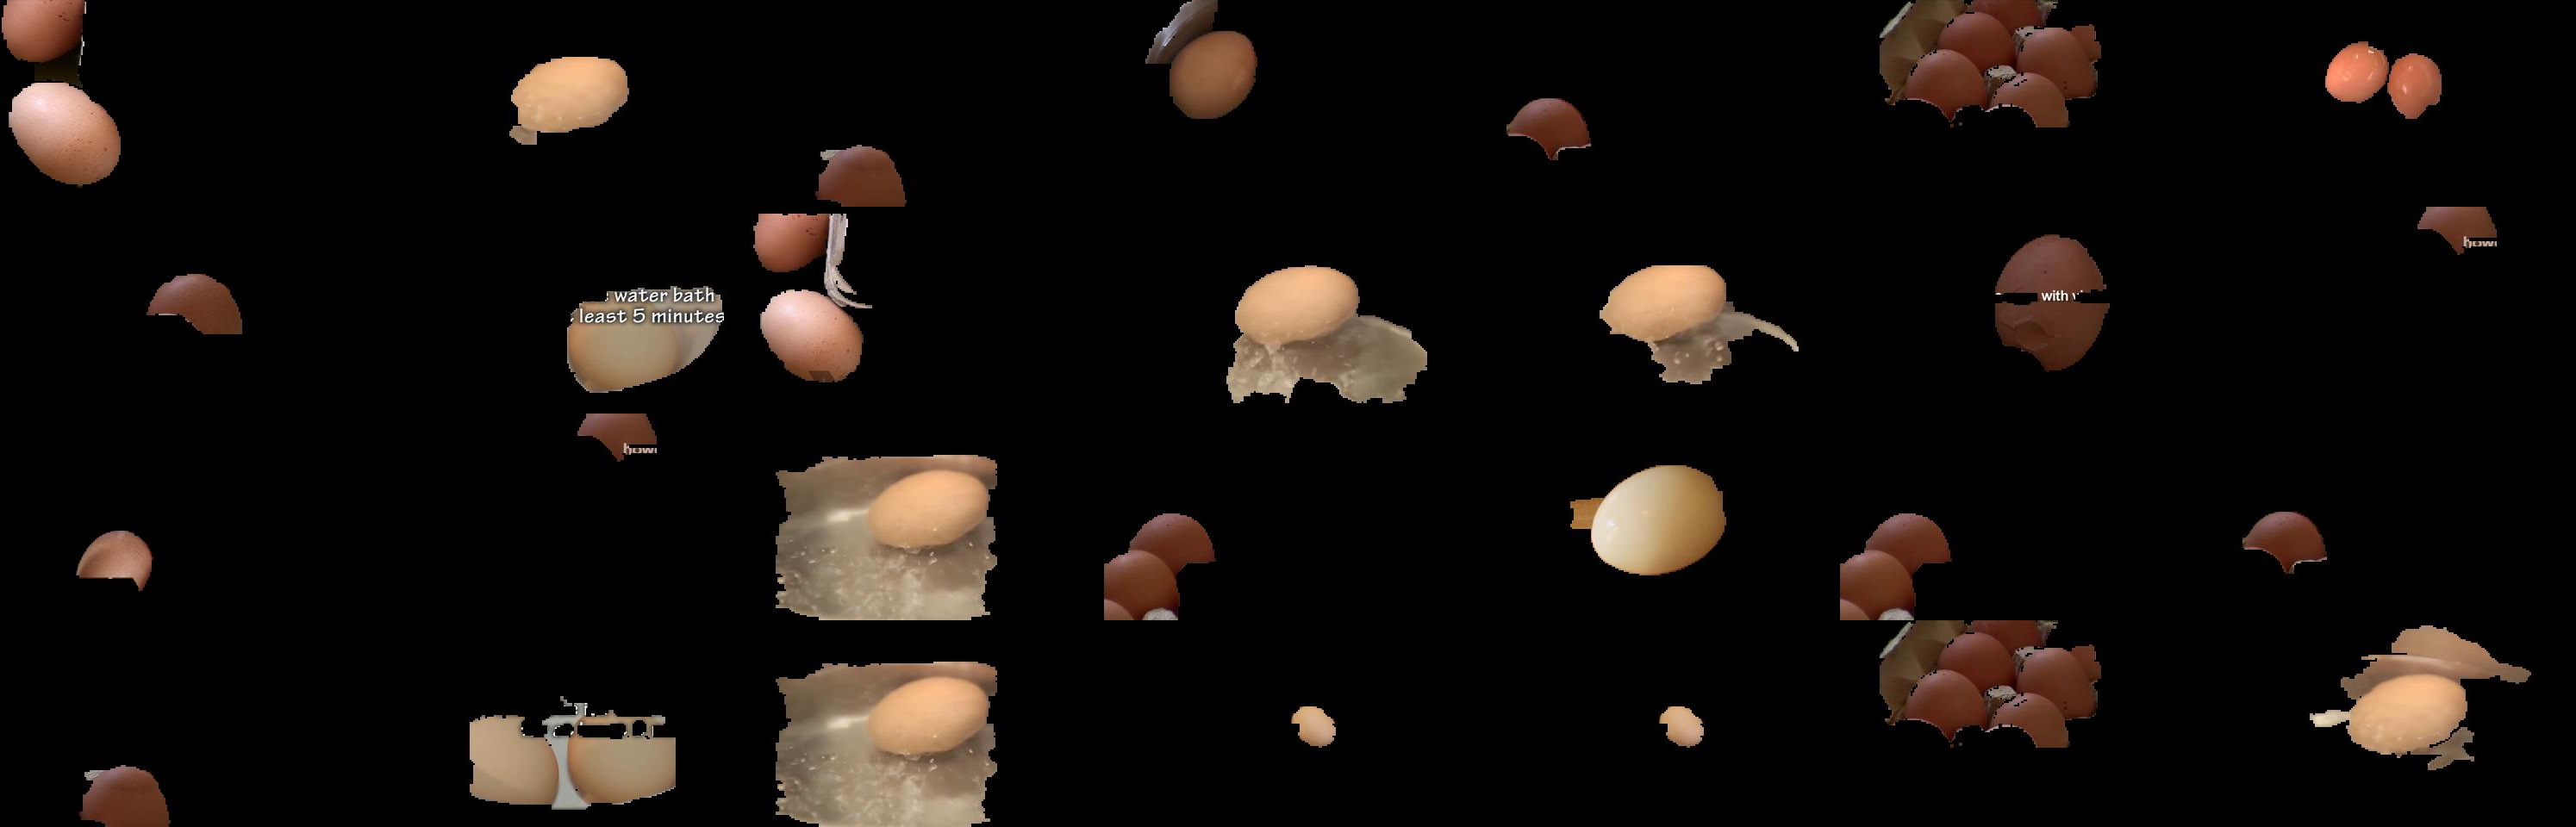
\includegraphics[width=\textwidth]{im4.png}
%\caption{Cluster 2}
\end{subfigure}
\begin{subfigure}[b]{0.23\textwidth}
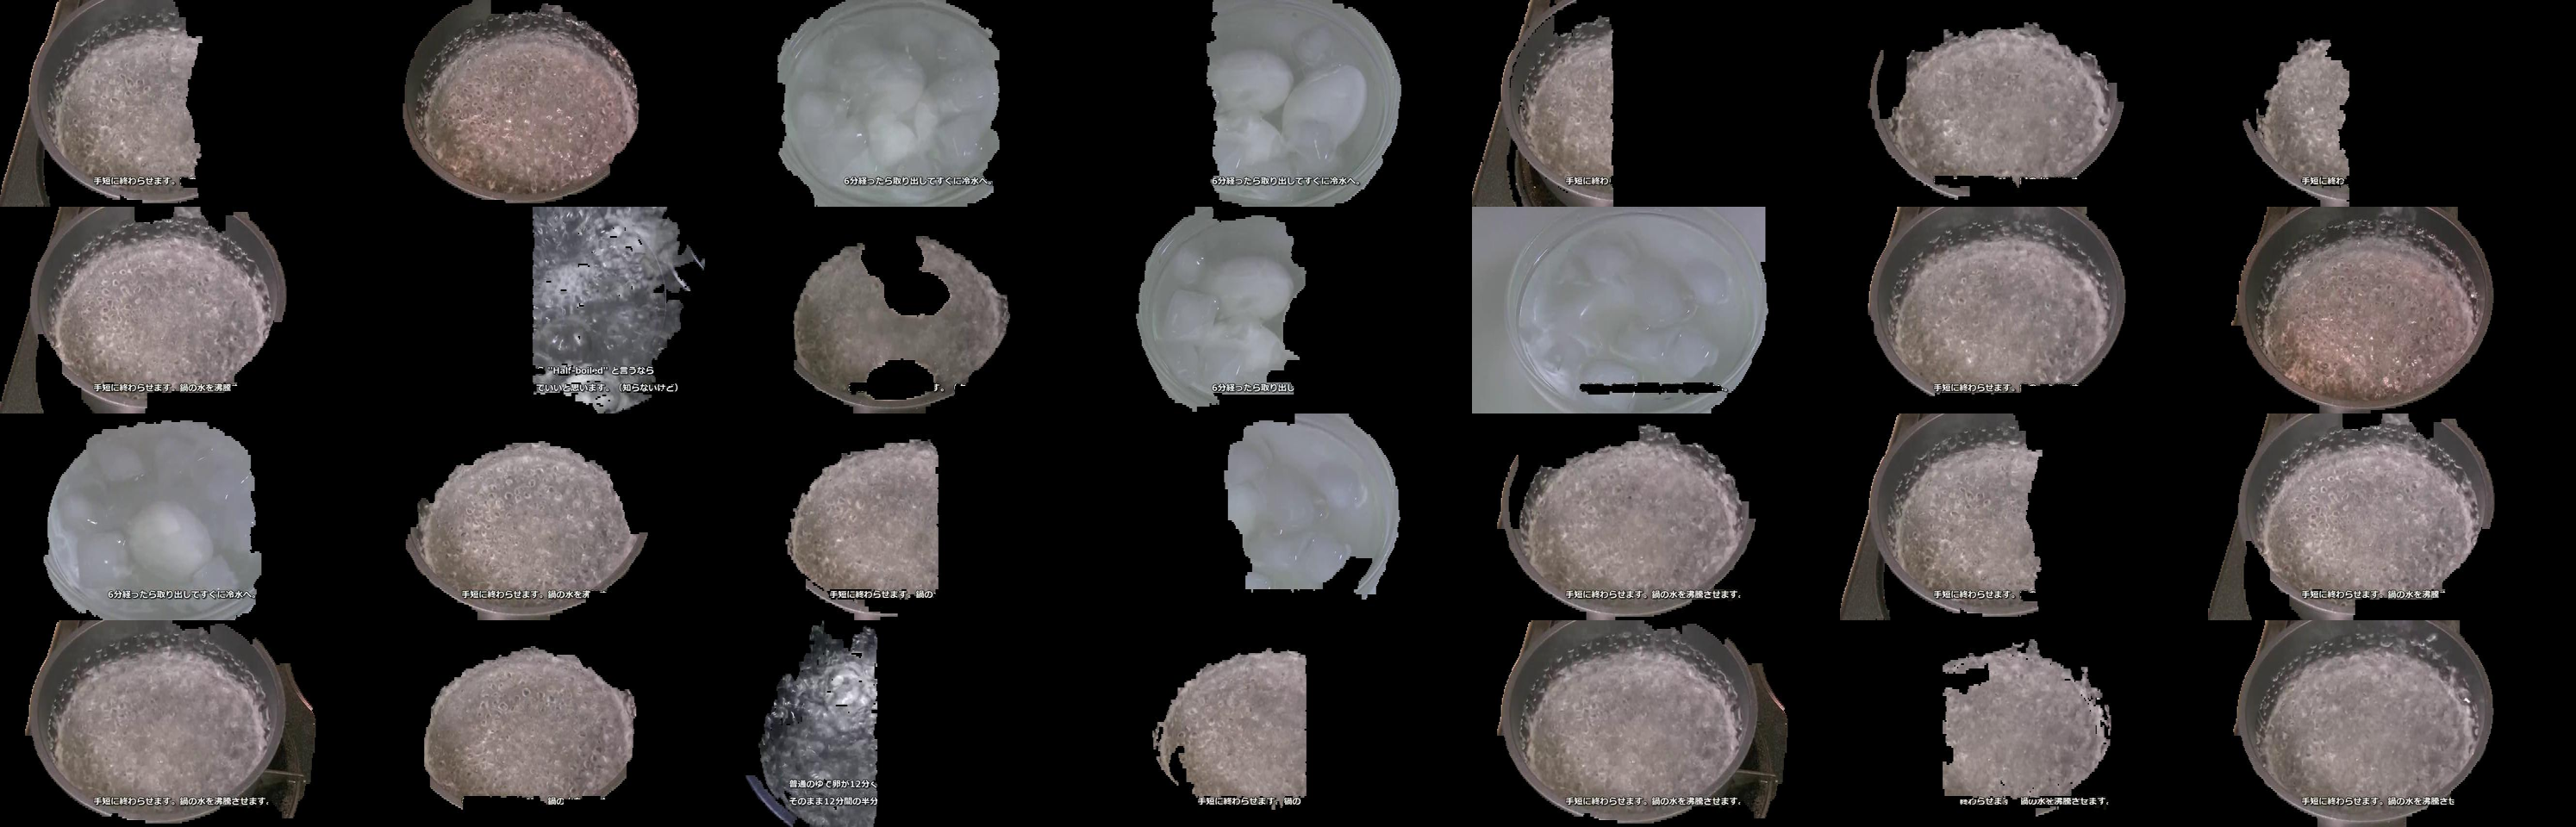
\includegraphics[width=\textwidth]{im5.png}
\end{subfigure}
~
\begin{subfigure}[b]{0.23\textwidth}
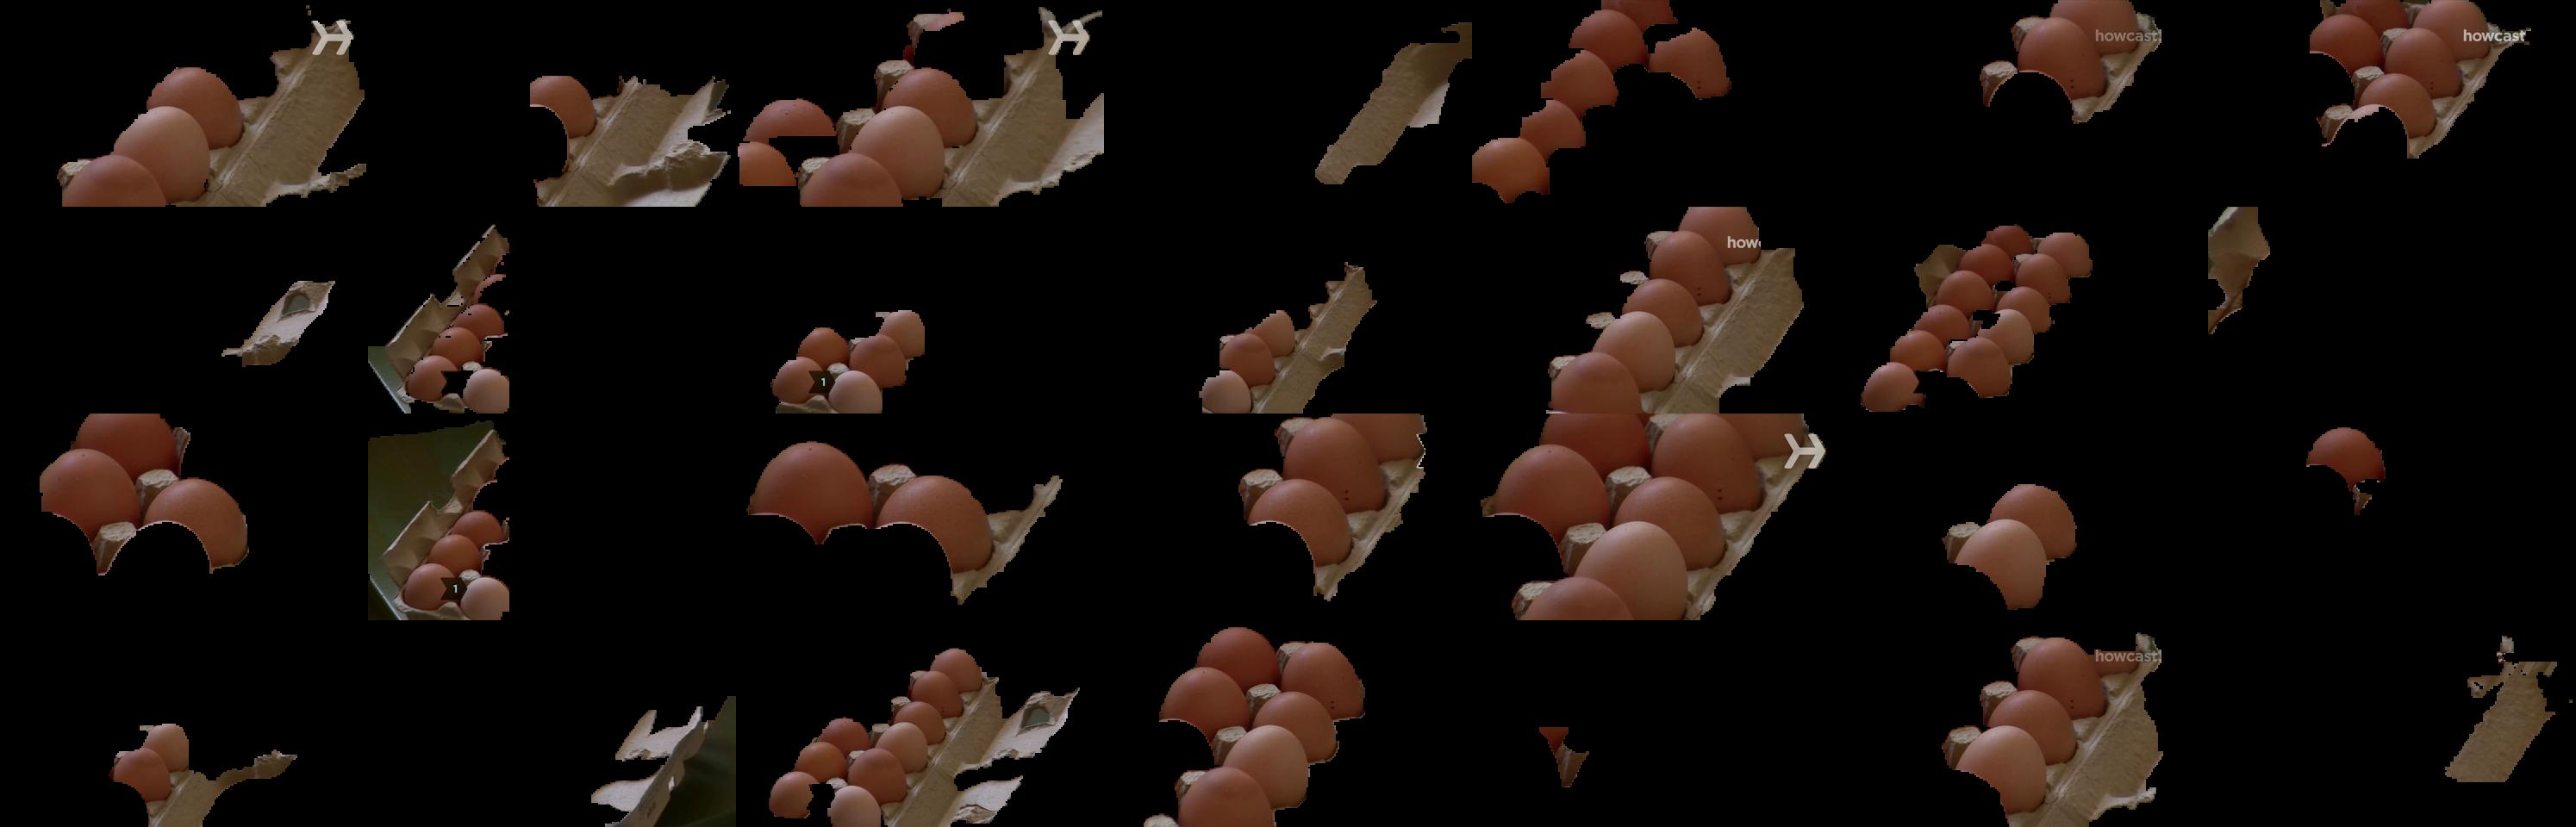
\includegraphics[width=\textwidth]{im7.png}
\end{subfigure}

\begin{subfigure}[b]{0.23\textwidth}
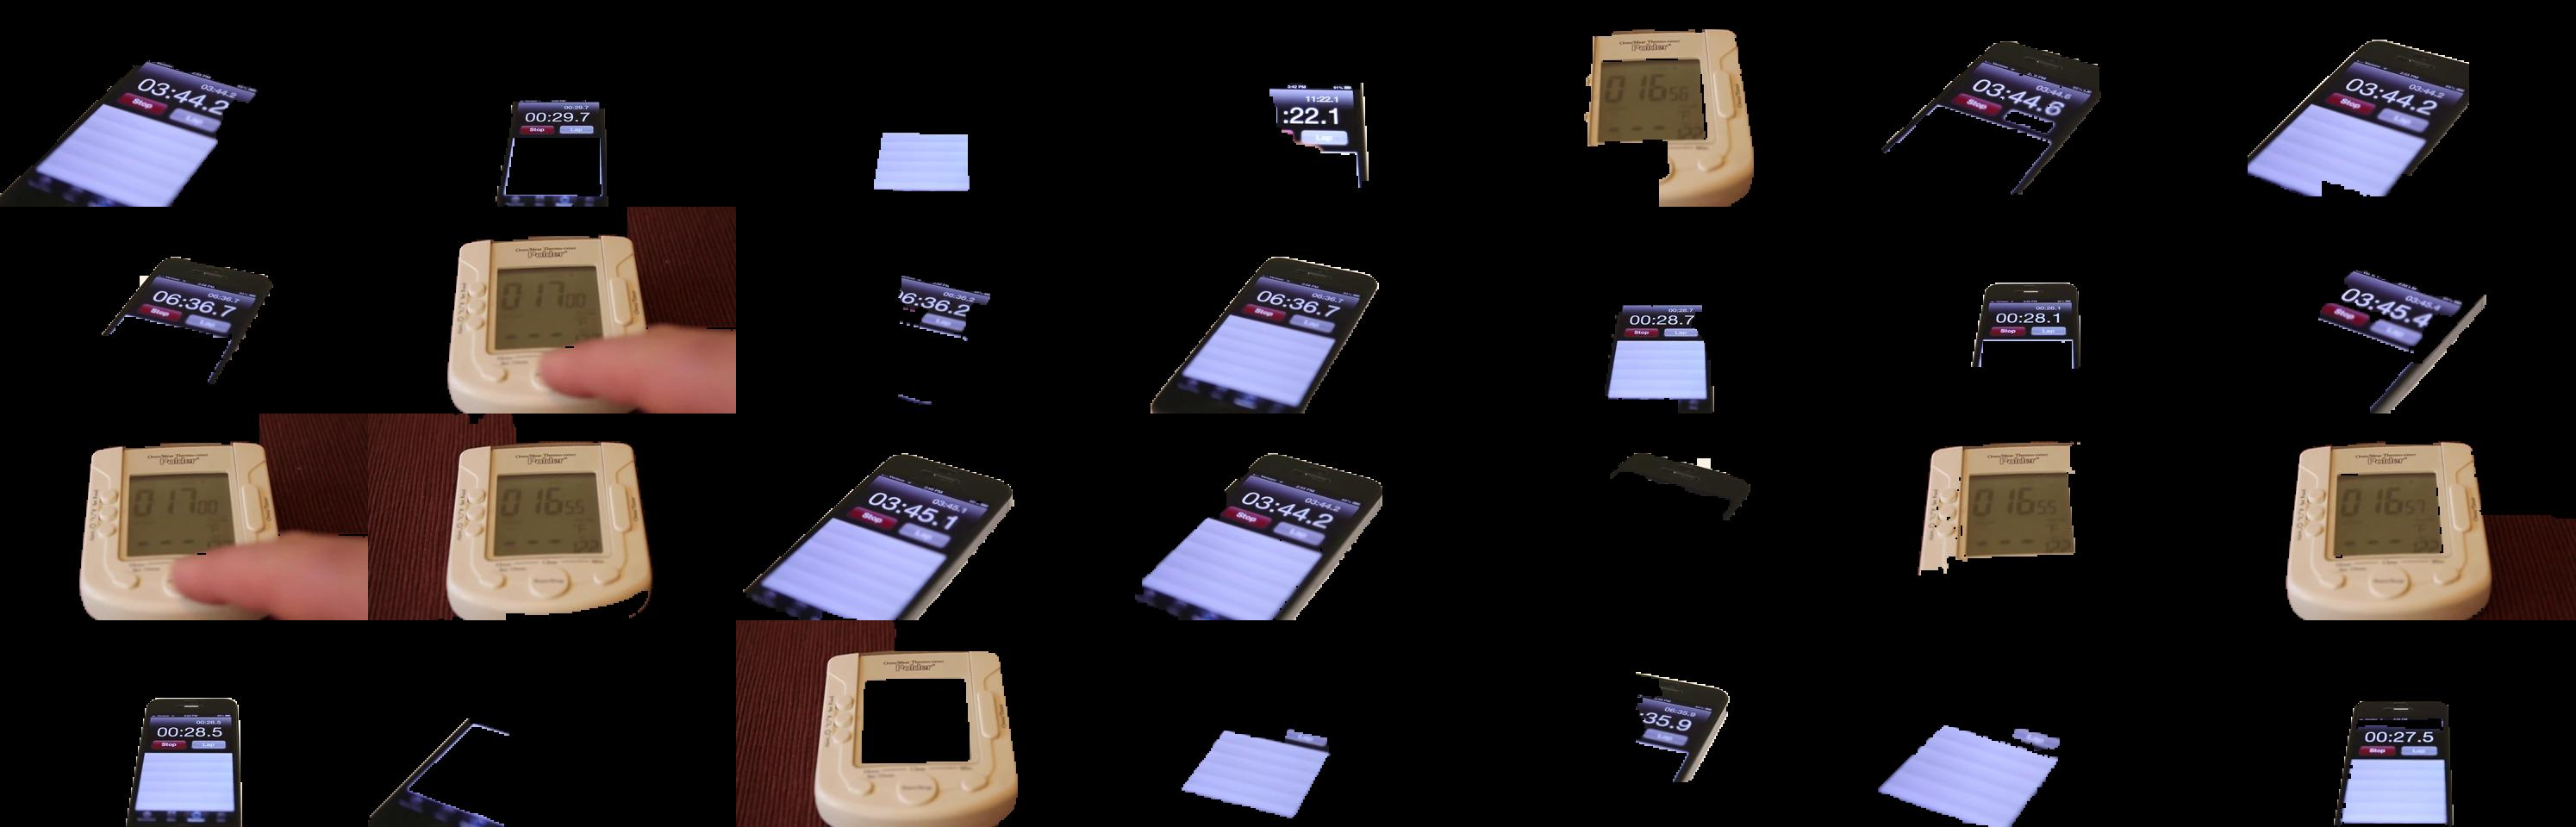
\includegraphics[width=\textwidth]{im8.png}
\end{subfigure}
~
\begin{subfigure}[b]{0.23\textwidth}
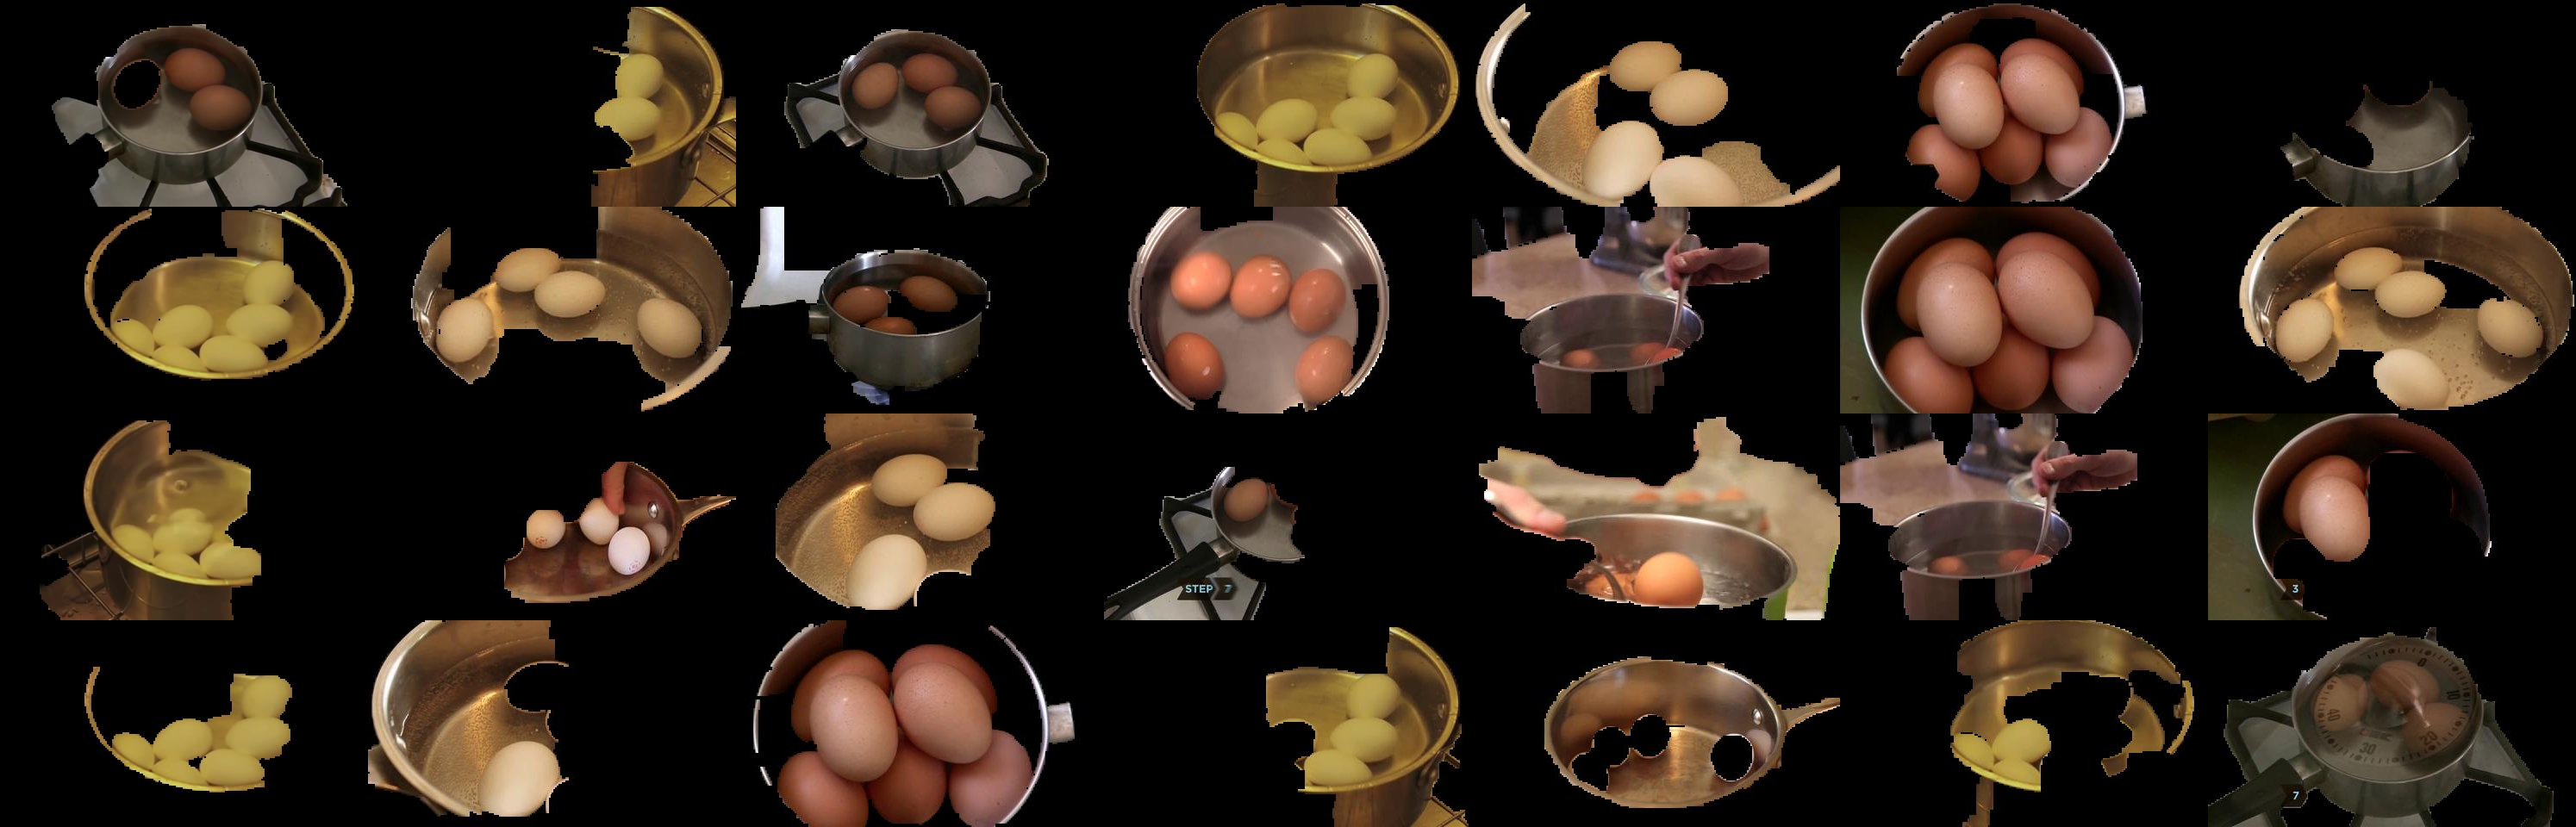
\includegraphics[width=\textwidth]{im10.png}
\end{subfigure}
\caption{Randomly selected images of randomly selected clusters learned for \emph{How to boil an egg?}}
\label{cvis}
\end{figure}
\subsection{Multi-Modal Representation via Learned Atoms}
